\section{数据科学导论部分}\label{SecDataScience}
\begin{center}
    Instructor: Sheng Yu
\end{center}

\begin{point}
    Road to Data Scientist
\end{point}

\begin{figure}[H]
    \centering
    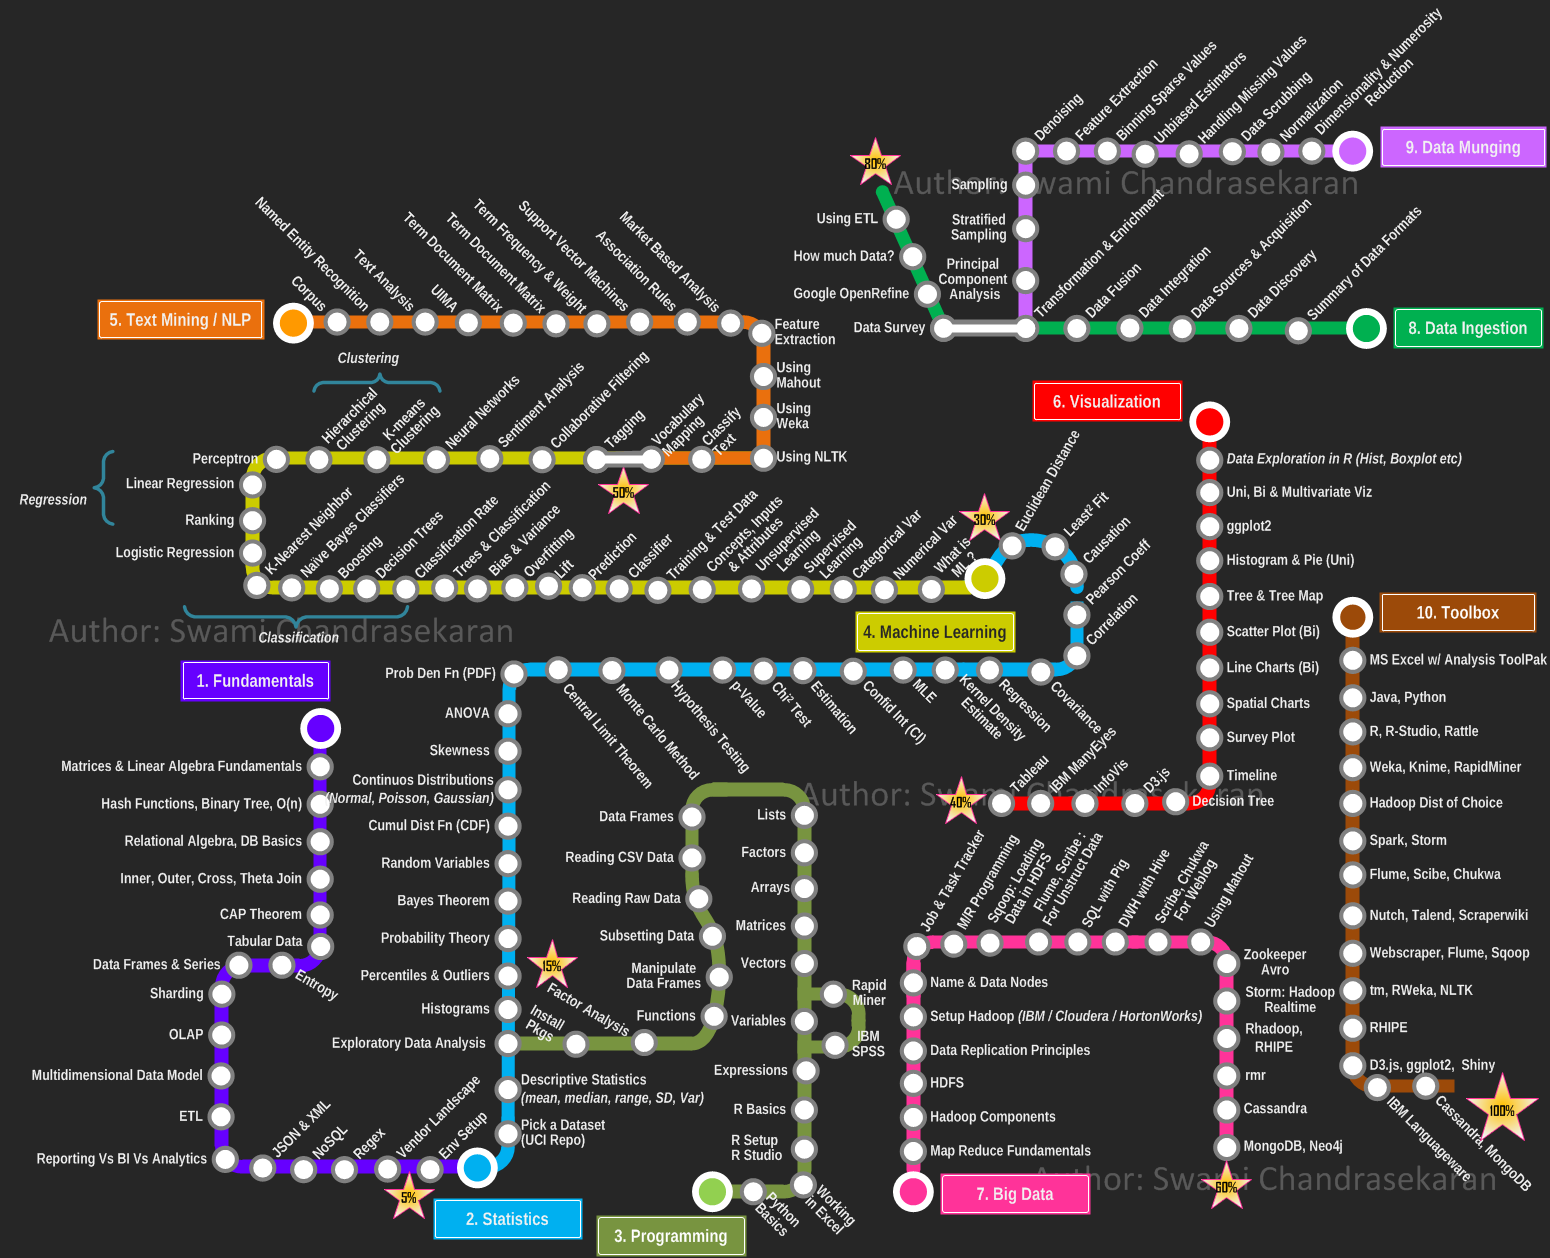
\includegraphics[width=\linewidth]{pic/RoadToDataScientist1.png}
    \caption{Road to Data Scientist}
    \label{RoadToDataScience}
\end{figure}


Comparison of \lstinline|R|, \lstinline|python|:focus on different aspects of `Statistics':
\begin{itemize}[topsep=2pt,itemsep=0pt]
    \item Differnece in programming philosophy: \lstinline|R| for data analysis and \lstinline|python| for data processing
    \item Difference in operating domain: \lstinline|R| for statistical programming while \lstinline|python| for general programming.
\end{itemize}



\subsection{Basic R. Manipulation}


\subsubsection{Installation and Maintenance of R.}

\noindent Installing and updating \lstinline|R.|: update by delete old version and install new version.
\begin{itemize}[topsep=2pt,itemsep=0pt]
    \item In CRAN (The Comprehensive \lstinline|R| Archive Network):\index{CRAN (The Comprehensive R Archive Network)} \url{https://cran.r-project.org}
    \item In Mirror@TUNA: \url{https://mirrors.tuna.tsinghua.edu.cn/CRAN}
\end{itemize}

\noindent Installing and updating RStudio: \url{https://www.rstudio.com}


\noindent Running \lstinline|R.| command:
\begin{itemize}[topsep=2pt,itemsep=0pt]
    \item In \lstinline|R.| GUI\index{GUI (Graphical User Interface)};
    \item In \lstinline|R.| command line terminal;
    \item \lstinline|R. CMD BATCH|;
    \item \lstinline|Rscript|;
        \begin{itemize}[topsep=2pt,itemsep=0pt]
        \item Use \lstinline|>| to redirect output(overwrite);
        \item Use \lstinline|>>| to append output.
        \end{itemize}
\end{itemize}



\noindent \lstinline|R.| package library: packages are collection of \lstinline|R.| functions (as well as test data and sample code).
\begin{itemize}[topsep=2pt,itemsep=0pt]
    \item \lstinline|.libPaths()| show package library location\footnote{Unlike in \lstinline|C| or \lstinline|python| where \lstinline|.| is an operator, \lstinline|.| in \lstinline|R.| is just a common character, without special meaning.
    
    This feature can be used in naming self-defined functions: use \lstinline|.FUN_NAME1| for within-project function while \lstinline|FUN_NAME2| for external interface.} ;
    \item \lstinline|library('PACKAGE_NAME1','PACKAGE_NAME2',...)| load packages.
    \item \lstinline|install.packages('PACKAGE_NAME1','PACKAGE_NAME2',...)| install package from CRAN/mirrors;
    \item \lstinline|installed.packages()| show all installed packages;
    \item \lstinline|updata.packages(checkBuilt = TRUE, ask = FALSE)| update installed packages;
\end{itemize}

\noindent Working Directory manipulation:
\begin{itemize}[topsep=2pt,itemsep=0pt]
    \item \lstinline|getwd()| get current working directory;
    \item \lstinline|setwd('TARGET_PATH')| set working directory as an existing path.  
\end{itemize}

\noindent Recommended \lstinline|R.| project organization: working directory organized like
\begin{itemize}[topsep=2pt,itemsep=0pt]
    \item \lstinline|data/| folder for structured original dataset;
    \item \lstinline|result/| folder for output result;
    \item \lstinline|presentation/| folder for result representing slides/reports/etc.;
    \item \lstinline|.r| project file $ \times n $.
\end{itemize}



\subsubsection{Data Manipulation in R.}

\begin{point}
    Looking for help/example of function:
\end{point}

\begin{itemize}[topsep=2pt,itemsep=0pt]
    \item \lstinline|?FUN_NAME()|;
    \item \lstinline|help('FUN_NAME')|;
\end{itemize}





\begin{point}
    Atomic Classes
\end{point}
\begin{itemize}[topsep=2pt,itemsep=0pt]
    \item \lstinline|'abc'| Character;
    \item \lstinline|3L| Integer;
    \item \lstinline|2.4| Numeric;
    \item \lstinline|TRUE,FALSE,T,F| Logical;
    \item Special types: \lstinline|NA|, \lstinline|NaN|, \lstinline|NULL|, \lstinline|Inf|
\end{itemize}

\begin{point}
    Operators
\end{point}
\begin{itemize}[topsep=2pt,itemsep=0pt]
    \item Numerical Operators: \lstinline|+|,\lstinline|-|,\lstinline|*|(multiply by column),\lstinline|/|,\lstinline|%*%|(matrix multiply),\lstinline|^|;
    \item Logical Operators: \lstinline|==|,etc.; \lstinline|&| and \lstinline{|} for common operator, \lstinline|&&| and \lstinline{||} for comparing the first element;
    \item Round a numeric:
    \begin{itemize}[topsep=2pt,itemsep=0pt]
        \item \lstinline|as.integer()|, round towards 0
        \item \lstinline|trunc()|
        \item \lstinline|ceiling()|
        \item \lstinline|floor()|
        \item \lstinline|round(NUMBER_TO_ROUND,digits = DIGITS)|
    \end{itemize}
    
        
\end{itemize}


\begin{point}
    Data Structure
\end{point}
\begin{itemize}[topsep=2pt,itemsep=0pt]
    \item Vector: Column vector is the \textbf{basic} data structure in \lstinline|R.| (scalar is length=1 vector).
    
    Only data of the same class can be held in one vector.
    
    Initialization:
    \begin{itemize}[topsep=2pt,itemsep=0pt]
        \item Ordinary way: 
        \begin{itemize}[topsep=2pt,itemsep=0pt]
            \item \lstinline|c(1,2,3)|, \lstinline|c(T,FALSE,TRUE)|, \lstinline|c('a',NA,'b')|
            \item \lstinline|vector(mode = MODE,length = LENGTH)|
        \end{itemize}
        
        where \lstinline|c()| for `combine'; 
        
        \lstinline|c()| combines all things into one vector, e.g. \lstinline|c(c(1,2,3),c(1,2))=(1,2,3,4,5)|.
        \item Sequence vector: 
        \begin{itemize}[topsep=2pt,itemsep=0pt]
            \item \lstinline|1:3.5=c(1,2,3)|, \lstinline|3:1=c(3,2,1)|
            \item \lstinline|seq(from, to ,by, length.out)|, \lstinline|length.out| for total vector length;
            \item \lstinline|rep(SEQ_TO_REP, times, lenght.out ,each)|, used in $ k $-fold cross validation labelling.
        \end{itemize}
    \end{itemize}
    
    Operations:
    \begin{itemize}[topsep=2pt,itemsep=0pt]
        \item between vectors of different length \lstinline|SHORT| and \lstinline|LONG|: First \lstinline|SHORT <- rep(SHORT,|\\\lstinline| length.out=length(LONG))|. Then operate \lstinline|SHORT| and \lstinline|LONG|.
        \item Element access: \lstinline|a[i]|
    \end{itemize}
    
         
    \fbox{
        \begin{minipage}{0.9\linewidth}

    \textbf{Vectorized Operation}: All operation in \lstinline|R.| are based on vector, and vectorized operation is \textbf{Parallel Arithmetic}, which is \textbf{much faster} than loop such as \lstinline|for| $ \longrightarrow $ Consider using vectorized opertion when writing code for \textbf{Speed}! 
        \end{minipage}
    }

    \item Factor: A special kind of `vector' in \lstinline|R.|, used to label discrete categorical data.\footnote{Factor vector is stored as integer vector.}
    
    Initialization:

    \lstinline|factor(FACTOR_SEQ, levels = FACTOR_LEVEL, labels = ...)|, \lstinline|FACTOR_LEVEL| is the `rank' of each factor, \lstinline|labels| is the `tag' of levels. 

    \item Matrix: Only data of the same class can be held in one matrix.
    
    Initilaization:
    
    \lstinline|matrix(DATA_SEQ, nrow, ncol, byrow = FALSE|
    
    If \lstinline|length(DATA_SEQ) < nrow*ncol|, then \lstinline|DATA_SEQ| is repeated. Default: fill by column (because matrix is stored by column).

    Operation:
    \begin{itemize}[topsep=2pt,itemsep=0pt]
        \item Common operators \lstinline|+-*/^| etc. operate in column-by-column mode (vectorized operation).
        \item Binding matrix: \lstinline|cbind| for \lstinline|[A,B]| and \lstinline|rbind| for \lstinline|[A;B]|
        \item Transpose: \lstinline|t()|
        \item Matrix multiplication: \lstinline|%*%|
        \item Inverse matrix: \lstinline|solve()| (The essence of inversion is solving linear equations)
        \item Diagonal matrix:
        \begin{itemize}[topsep=2pt,itemsep=0pt]
            \item \lstinline|diag(VECTOR)| returns a matrix $ \mathrm{diag}\{ $\lstinline|VECTOR|$ \} $
            \item \lstinline|diag(MATRIX)| returns the diagonal element vector
        \end{itemize}
        \item Element access: \lstinline|a[i,j]|, \lstinline|a$OBJECT_NAME|
        \item Dimension of matrix: \lstinline|dim()|, \lstinline|nrow()|, \lstinline|ncol()|
    \end{itemize}
    
    \item List: A pack containing various datatype
    
    Initialization: \lstinline|list(OBJECT1,OBJECT2,...)|

    Element access: \lstinline|a[[i]]|
    \item \lstinline|data.frame|: `Mixture' of matrix and list. \lstinline|data.frame| is actually a kind of list(with some constraint), organized in the shape of matrix (but allowing different datatype for different columns, each column is a list object).
    
    Each column of \lstinline|data.frame| has name: \lstinline|names(DATA_FRAME)|, \lstinline|colnames(DATA_FRAME)|

    \item Element access: \lstinline|a[i,j]|, \lstinline|a[[i]]|, \lstinline|a$COL_NAME|
\end{itemize}

    

    
    
        

    





    




     




    

    








